\documentclass[aspectratio=1610]{beamer}

\usepackage{amsmath}
\usepackage{multirow}
\usepackage{url}
\usepackage{hyperref}

\hypersetup{
colorlinks=false,
}

\usepackage{listings,calc,graphicx}

\title % [short title] (optional, use only with long paper titles)
{CPSC 1000: Introduction to Computer Science}

\subtitle{Reading the state of a button} % (optional)

\author{Robert Benkoczi, C556\\\url{robert.benkoczi@uleth.ca}}
\date{2-Oct-2018\\(Week 4)}

% for figures created with IPE
%\pdfpagebox5

\lstloadlanguages{C}
\lstset{language=C,tabsize=2,aboveskip=-22pt,belowskip=-22pt,keepspaces,
  basicstyle=\small\ttfamily,}


\begin{document}

\begin{frame}[plain]
\titlepage
\end{frame}

%%%%%%

\begin{frame}[t,plain]{Simplest user input}

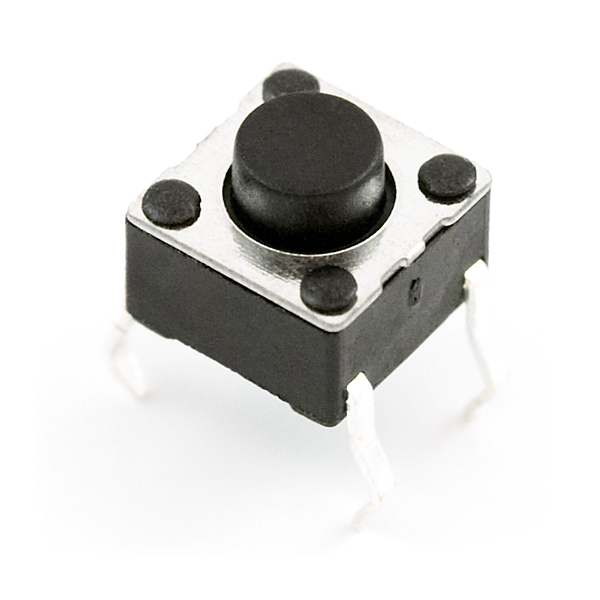
\includegraphics[width=0.3\textwidth]{figs/2-button.jpg}
\hfill
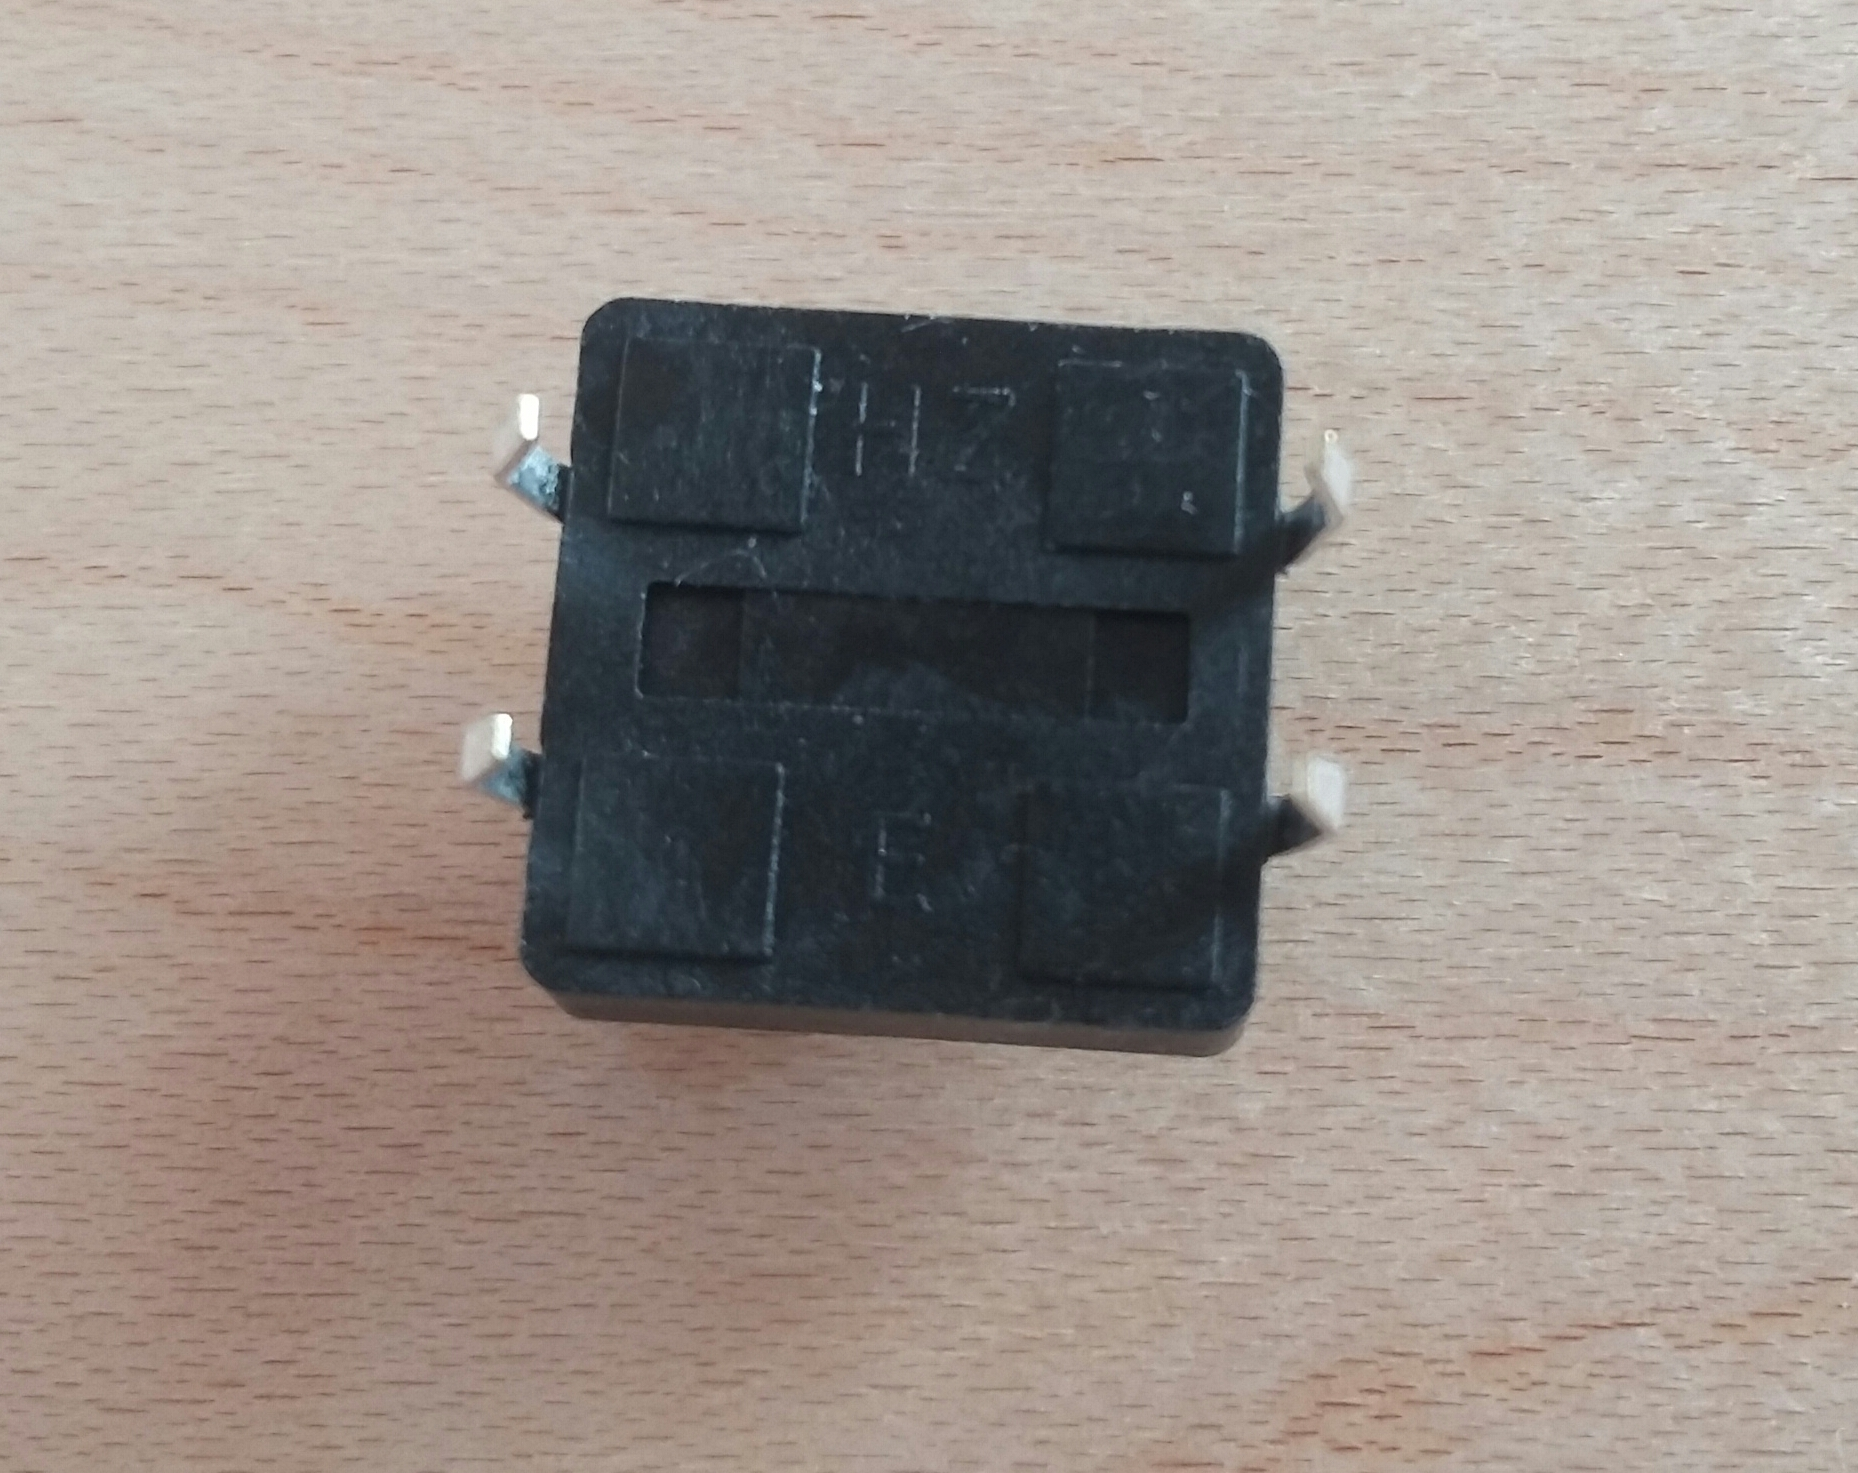
\includegraphics[width=0.4\textwidth]{figs/2-button_back.jpg}
\hfill ~
\end{frame}


%%%%%%

\begin{frame}[t,plain]{Digital input}

\begin{itemize}
\item pinMode(digital\_pin, INPUT)

\bigskip
\item Connect the input pin to bit 1:

\vspace*{0.4\textheight}
\item Connect the input pin to bit 0:
\end{itemize}
\end{frame}


%%%%%%

\begin{frame}[t,plain]{Digital input}
\begin{itemize}
\item Connect the input pin to 0 when pressed and to 1 when depressed.

\vspace*{.4\textheight}
\item ... using a resistor.
\end{itemize}
\end{frame}


%%%%%%

\begin{frame}[t,plain]{Digital input}
\begin{itemize}
\item Connect the input pin to 1 when pressed and to 0 when depressed
  (using a resistor).
\end{itemize}
\end{frame}

%%%%%%%%

\begin{frame}[t,plain]{Programming}
\begin{itemize}
\item pinMode(digital\_pin, INPUT);

\item digitalRead(digital\_pin)

\bigskip
\item The return value for pressed/depressed button state depends on
  the type of circuit.

\bigskip
\item If pin is not connected to Vcc or GND, the return value is
  either HIGH or LOW non-deterministically.
\end{itemize}
\end{frame}


%%%%%%%%

\begin{frame}[t,plain]{Programming, built-in pull-up}
\begin{itemize}
\item pinMode(digital\_pin, INPUT\_PULLUP);

\item digitalRead(digital\_pin): returns HIGH unless pin connected to GND.
\end{itemize}
\end{frame}


%%%%%%%%

\begin{frame}[t,plain]{Exercises}
Configure digital pin 7 with the built-in pull-up resistor. Draw a
circuit that allows detecting the pressing of a button. What is the
corresponding Arduino code?
\end{frame}

\end{document}
